% !TEX root = ../thesis.tex
\chapter{Experimenty}
\label{chap:experiments}

Jak již bylo zmíněno v předchozích sekcích, tak velmi významným problémem je psychologický faktor ztráty hlasu. To sebou nese i na první pohled neúplně zřejmý problém, kterým je obtížné získání získání řečníka po TL, který je ochotný spolupracovat na výzkumu.

Jedním z možných řešení je, že se výzkumníci sami naučí používat jednu z výše  \todo{TBD}{[c4l1]})zmíněných metod produkce řeči. Pro účely našeho výzkumu a rámec této práce by se jednalo o elektrolarynx. I když se tato možnost jeví poměrně jednoduše, tak zdání klame. Přestože je zdravý řečník schopen obstojně mluvit (pomocí EL), za relativně krátkou dobu tak k tomu, aby produkovaná řeč svými parametry odpovídala řečníkovi po TL, je potřeba relativně dlouhá doba.

Pro účely našeo výzkumu se nám podařilo získat pouze jednoho zkušeného řečníka\footnote{Jedná se o ženu v důchodovém věku, která ale stále působí na akademické půdě a jednou za čas i přednáší.}, který podstoupil TL před cca 15 lety a EL používá aktivně každý den. Je to jediná možnost jak produkovat slyšitelnou řeč.

Díky spolupráci s tímto řečníkem jsme byli schopni získat cca 15 hodin promluv (více o získaných datech v \ref{chap:experiments:analysis} a \ref{chap:experiments:normalization}), které byly použity pro všechny dosavadní experimenty. Z pohledu standardních obecných systémů rozpoznávání řeči se to může jevit jako velmi malé množství, ale jak ukáží následné experimenty, tak to není velký problém. Jelikož už před prvními experimenty se jevilo jako prozaičtější vytvářet individuální modely pro každého řečníka a výsledky experimentů toto jen podpořily.

Při rozhovorech s řečníkem se potvrdil psychický dopad ztráty hlasu na člověka po TL. Konkrétní osoba ještě dlouhá léta po operaci nebyla schopna telefonovat natož mluvit na veřejnosti. Kvalita života se tímto velmi snížila a trvalo prý velmi dlouho dobu, než se daná osoba odvážila i jen odpovědět na nečekaný telefonní hovor.

V následujícím textu si přiblížime a zanalyzujeme pořízená data (\ref{chap:experiments:analysis}), dále popíšeme důvody normalizace dat a porovnáme schopnosti člověka a stroje (\ref{chap:experiments:normalization}). V sekci \ref{chap:experiments:poc} rozebereme prvotní ověřovací experimenty s upravenámi daty a v sekci \ref{chap:experiments:durationmodels} představíme výsledky modelů zohledňujících i délku fónému.

% Při konzultacích s pacienty vyšlo najevo, že psychická stránka je velmi důležitá a někdy to může věst až k paralýze (v obrazném slova smyslu) kdy ti lidé nebyli schopni třeba telefonovat. Takže systém, který by sice neřešil kompletní problematiku náhrady/rehabilitace řeči by mohl být užitečný.

% !TEX root = ../thesis.tex
\section{Analýza dat a první modely}
\label{chap:experiments:analysis}

\begin{itemize}
  \item popis jak byla data získána
  \item informace o datech (frakvenční rozsah, atp.)
  \item prvotní experimenty k určení parametrů modelu
  \item popsat výsledky, výsledky převážně na HTK (HMM + GMM)
\end{itemize}

% \csvautotabular{./ch4-experiments/test.csv}

\begin{table}[htpb]
  \centering
  \def\arraystretch{1.5}
  \pgfplotstabletypeset[
    col sep=comma,
    string type,
    columns/model/.style={column name=Model, column type={|c}},
    columns/8k/.style={column name=8 kHz $[\%]$, column type={|r}},
    columns/16k/.style={column name=16 kHz $[\%]$, column type={|r|}},
    every head row/.style={before row={
      \hline
      & \multicolumn{2}{c|}{WER} \\
    },after row=\hline},
    every last row/.style={after row=\hline},
  ]{./ch4-experiments/tabs/01-frequency.csv}
  \caption{Vliv frekvence na kvalitu modelu.}
\end{table}

% !TEX root = ../thesis.tex
\section{Porovnání člověk vs. stroj}
\label{chap:experiments:normalization}

Z experimentů provedených v části \ref{chap:experiments:analysis} vyplynula potřeba rozšířit korpus řečových dat. V části \ref{chap:experiments:analysis:reduction} se ukázalo, že v určitých případech jsou neznělé fonémy produkovány jako znělé. Pro lepší porozumnění tohoto jevu je nezbytné, aby řecový korpus obsahoval co možná nejvíce promluv obsahující slova slova s odlišným významem, ale lišící se pouze ve znělosti jedonho fonému.

Tato část se zaměřuje na získání takových to slov a experimentů s těmito slovy. Hlavním experimentem je porovnání schopností člověka tato slova od sebe odlišit a stroje. Na základě poznatků z tohoto experimentu jsou nabrženy úpravy, které mají sloužit k zlepšení systémů rozpoznávání řeči.

\subsection{Rozšíření řečového korpusu}
\label{chap:experiments:normalization:corpus}

Před samotným nahráváním bylo nezbytné vybrat co možná nejvíce dvojic slov, které se liší významem a ve znělosti právě jednoho fonému. Příkladem může být dvojice slov \textit{kosa} + \textit{koza} nebo \textit{přibít} + \textit{přibít}. Algoritmus výběru slov je následující:

\begin{enumerate}
  \item načtení dat (slovník, párové fonémy)
  \item shluknutí všech slov vedoucích ke stejné transckripci
  \item zkombinování všech transkripcí do dvojic
  \item nalezení dvojic transkripcí, které se liší právě ve znělosti jednoho fonému\footnote{Konkrétně algoritmus vzájemně porovná obě slova a najde rozdílné fonémy. Pokud tyto rozdíly odpovídají některé z dvojic párových fonémů, tak je dvojice přijata.}
  \item výběr dvojic slov na základě vybraných transkripcí
\end{enumerate}

Vstupem je tedy slovník obsahující slova a jejich fonetický přepis, dále pak dvojice fonémů (znělý + neznělý). Jako slovník posloužil seznam slov s fonetickými přepisy pocházející z jazykového modelu obsahující 1,2 milionu slov. Pomocí výše zmíněného algoritmu se podařilo nalézt $160$ párů slov lišících se znělostí právě jednoho fonému, celkem tedy $320$ slov. Ke každému nalezenému slovu byla následně vybrána minimálně jedna věta obsahující toto slovo (ale nikoli druhé slovo z dvojice), těchto vět je pak $418$. Příklad vybraných vět je níže

\begin{verbatim}
  Zkoušel jsem to několikrát, ale pokaždé padla kosa na kámen.
  Do basy nemusí, vlk žere, koza žije.
\end{verbatim}

Vybraná slova a věty jsou základem pro druhou etapu nahrávání. Nahrávání se zhostil stejný řečník jako v případě té první (viz část \ref{chap:experiments:analysis:corpus}). Samotné nahrávání bylo rozděleno do dvou samostatných sezení, mající mezi sebou týdenní rozestup. Oproti první etapě probíhalo nahrávání v odhlučněné nahrávácí komoře za pomocí profesionálního nahrávacího zařízení. Mikrofon byl od úst řečníka vzdálen přibližně 15 cm, protože byl použit studiový mikrofon, který kvůli své velikosti už z podstaty není možné přiložit přímo na tvář jako v případě první série nahrávání. K nahrávání byl použit speciální software, který kontroloval zda každá nahrávka splňuje určité parametry. Každá nahrávka musí mít na svém začátku a konci minimálně $0,5\ s$ ticha a zároveň celá nahrávka nesmí být příliš tichá a zároveň přebuzená (kontrolováno pomocí energie). Pokud nahrávka nesplňovala definované parametry, tak byla zamítnuta a řečník musel promluvu zopakovat.

V částu \ref{chap:experiments:analysis:corpus} je zmíněno, že je nezbytné provést anotaci nahrávek, aby mohl být korpus kompletní. Samotná anotace je navíc relativně zdlouhavý proces, a proto je dobré pořídit přesné promluvy vybraných slov a vět. K tomu slouží další z funkcí nahrávacího softwaru, který řečníkovi vždy ukáže text, který je potřeba vyslovit. Společně s audio záznamem je pak uložen i tento text. K dispozici je tedy nahrávka a její \uv{přepis}. Nicméně samotný řečník často může udělat chybu aniž by si toho všiml (např. záměna podobných slov apod.) a software nijak nekontroluje co bylo ve skutečnosti vysloveno. Z tohoto důvodu je nahrávání přítomen operátor, který poslouchá co bylo řečeno a v případě potřeby zamítné nahrávku. Řečník následně musí promluvu opakovat dokud nahrávka neodpovídá požadovaným parametrům a zároveň je její obsah správný.

Na obr. \ref{fig:experiments:normalization:word} a \ref{fig:experiments:normalization:sentence} jsou ukázky audio záznamu slova \uv{kosa} a věty \uv{Zkoušel jsem to několikrát, ale pokaždé padla kosa na kámen.}. Pokud se nahrávky porovnají s daty získanými v první etapě (obr. \ref{fig:experiments:analysis:el_speech}), tak hlavním rozdílem je vyšší kvalita nahrávek, zejména vyšší amplituda nahrávek. Ze zobrazených spektrogramů je zřejmé, že šum je přítomen v podobném spektru a intenzitě jako u předchozích nahrávek. Rozdíl je zejména v nižších frekvencích řeči, které jsou na spektrogramu výraznější. Přestože se jedná o stejného řečníka, tak zaznamenaná řeč nemá úplně identické parametry. Hlavním důvodem bude nepochybně změna nahrávací aparatury a procesu nahrávání. Nezanedbatelný vliv bude mít i relativní nestálost prametrů EL řeči, zvlášť v delším časovém období. Kvalita a parametry EL řeči je totiž velmi závisle na typu a pozici elektrolarynxu.

\begin{figure}[hbpt]
  \centering
  \includegraphics[width=0.9\textwidth]{./ch4-experiments/img/energy_spec_word.png}
  \caption{Průběh a spektrogram slova \uv{kosa} s společně s vyznačenou energií EL promluvy.}
  \label{fig:experiments:normalization:word}
\end{figure}

\begin{figure}[hbpt]
  \centering
  \includegraphics[width=0.9\textwidth]{./ch4-experiments/img/energy_spec_sentence.png}
  \caption{Průběh a spektrogram promluvy obsahující slovo \uv{kosa} a vyznačenou energií EL promluvy.}
  \label{fig:experiments:normalization:sentence}
\end{figure}

Celkem se v 2. etapě pořídila přibližně 1 hodina řečových dat. Celý korpus po 2. etapě tak obsahuje 11 hodin řečových dat, sestávajích z více než $5400$ vět a $320$ izolovaných slov.

\subsection{Vliv nových dat na kvalitě modelů}
\label{chap:experiments:normalization:corpus}

TBD




\begin{figure}[htpb]
  \centering
  \begin{subfigure}[b]{0.4\textwidth}
    \includegraphics[width=\textwidth]{./ch4-experiments/img/gmm-hmm.pdf}
    \caption{GMM-HMM}
    \label{fig:experiments:analysis:spectrogram:normal}
  \end{subfigure}
  %
  \begin{subfigure}[b]{0.4\textwidth}
    \includegraphics[width=\textwidth]{./ch4-experiments/img/dnn-hmm.pdf}
    \caption{DNN-HMM}
    \label{fig:experiments:analysis:spectrogram:el}
  \end{subfigure}
  \caption{Znázornění odlišného principu \textit{GMM-HMM} a \textit{DNN-HMM}.}
  \label{fig:experiments:analysis:spectrogram}
\end{figure}


Z dosažených výsledků vyplývá, že nová data jsou příliš odlišná od původních dat. Zároveň je těchto dat relativně malé množství, aby se mohly modely adaptovat. Na rozdíl v datech se můžeme koukat jako na změnu kanálu, která je příčinou změn v datech, protože řečník je stejný. V předchozím textu bylo zmíněno, že v rámci druhé etapy došlo ke změné nahrávací procedury. Tím byl pozměněn kanál a logicky výsledná zaznamenaná řeč má jiné parametry než ta v 1. etapě. Mezi další prvky, které mohou způsobit změnu kanálu může být prostředí, tedy jestli je řeč produkována uvnitř nějaké místnosti, či venku, jestli je na pozadí přítomen šum atp. K tomu, aby bylo možné použít všechna dostupná data, je potřeba eliminovat vliv kanálu. K jeho eliminaci je možné využít CMN, což je zkratka anglických slov Cepstral Mean Normalisation.

Zaznamenaný signál je možné popsat jako

\begin{equation}
  y\left[n\right] = x\left[n\right] \circledast h\left[n\right],
  \label{eq:experiments:normalization:convolution}
\end{equation}

\noindent kde $x\left[n\right]$ představuje vstupní signál, tedy řeč, a $h\left[n\right]$ odezva kanálu na jednotkový impulz. Zaznamenaný signál je pak jejich lineární konvolucí. Ve frekvenční oblasti pak rovnice \ref{q:experiments:normalization:convolution} zapsaná nýsledovně:

\begin{equation}
  Y\left[f\right] = X\left[f\right] \cdot H\left[f\right]
\end{equation}

\noindent Ve frekvenční oblasti se z konvuluce stalo násobění což značně zjednodušuje situaci. K odstranění vlivu kanálu je, ale ještě potřeba převést hodnoty do kepstrálná oblasti. To je realizováno pomocí logaritmu spektra

\begin{equation}
  Y\left[q\right] = \log\left(Y\left[f\right]\right) = \log\left(X\left[f\right] \cdot H\left[f\right]\right) = X\left[q\right] + H\left[q\right],
\end{equation}

\noindent kde $q$ představuje kepstrální koeficient. V kepstrální oblasti je vliv kanálu aditivní složkou výsledného záznamu. Problémem však je, že konkrétní hodnota vlivu kanálu je neznáma, protože k dispozici je pouze výsledný ovlivněný signál. Předpokládejme však, že vliv kanálu je stacionární\footnote{Jedná se sice o silný, ale logický předpoklad. Pokud se vztáhne k pořízenému řečovému korpusu, tak v rámci jedné etapy nahrávání, je proces nahrávání neměnný, tzn. je použita stejná aparatura a k nahrávání dochází vždy ve stejné místnosti.}, tak poté je možné každý frame nahrávky $i$ zapsat jako

\begin{equation}
  Y_i\left[q\right] = H\left[q\right] + X_i\left[q\right],
\end{equation}

\noindent kde $Y_i\left[q\right]$ představuje $i-\text{tý}$ frame kepstra $q$ nahrávky a $X_i\left[q\right]$ představuje $i-\text{tý}$ frame kepstra $q$ neovlivněné řeči. Z této rovnice je pak možné vypočítat střední hodnotu

\begin{equation}
  \frac{1}{N} \sum_i Y_i\left[q\right] = H\left[q\right] + \frac{1}{N} \sum_i X_i\left[q\right].
\end{equation}

\noindent Vliv kanálu je pak možné eliminovat odečtením střední hodnoty kepstra $q$ od aktuální hodnoty kepstra $Y_i\left[q\right]$

\begin{align}
  R_i\left[q\right] &= Y_i\left[q\right] - \dfrac{1}{N}\sum_{j} Y_j\left[q\right] \nonumber  \\
  &= H\left[q\right] + X_i\left[q\right] - \left( H\left[q\right] + \frac{1}{N} \sum_j X_j\left[q\right] \right) \nonumber  \\
  &= X_i\left[q\right] - \frac{1}{N} \sum_j X_j\left[q\right]
  \label{eq:experiments:normalization:cmn}
\end{align}

\noindent S pomocí rovnice \ref{eq:experiments:normalization:cmn} je možné odfiltrovat vliv kanálu a teoreticky by tak získat hodnoty kepstrálních koeficientů odpovídající nezkreslené řeči.

\subsection{Poslechový test}

\subsection{Výsledky porovnání}

\begin{itemize}
  \item popsat důvody proč potřebujeme další nahrávky (slova, která se liší znělostí)
  \item popsat algoritmus výberu slov/vět k nahrávání
  \item napsat něco o tom, že mezi nahráváními byl velký časový rozestup a taky se změnila technika nahráváními
  \item problém taky s tím, že první sada nahrávek je mnohem větší (10h) než ta nová (cca 30 min) a modely tak nefungovali na nových datech v testovací sade
  \item použití neuronovek (Kaldi)
  \item popis a výsledky experimentu \uv{člověk vs. stroj}
\end{itemize}

% !TEX root = ../thesis.tex
\section{Augmentace dat}
\label{chap:experiments:augmentation}

Poslechový test jasně uázal, že správné rozpoznání pronesené EL promluvy není lehký úkol ani pro člověka. Naprosto markantní význam hraje kontext. Ten velmi významně pomáhá, pokud některá část promluvy nebyla dobře rozumnět nebo bylo těžké ji porozumnět. Navíc, ze zkušeností získaných při pořizování řečového korpusu (části \ref{chap:experiments:analysis:corpus} a \ref{chap:experiments:normalization:corpus}), plyne, že EL řečník má tendenci mluvit ve spíše kratších dávkách slov, mezi kterými dělá drobné pauzy. V tomto případě pro člověka není problém udržet v povědomí kontext, ale stroji to může někdy způsobovat problémy. Otázkou tedy je, jak \uv{vylepšit} stroj tak, aby poskytoval lepší výsledky?

Ať se řečník snaží sebevíc, tak se současnými metodami rehabilitace hlasu (viz \ref{sec:cause:treatment}), se při ztrátě hlasivek část informace z produkované řeči ztrácí. Obnovit tuto informaci se snaží valná většina prezentovaných přístupů v části \textbf{TBD}. Ve valné většině případů se k tomu využívá obohacení modelu o artikulační data, nebo dokonce využití jen těchto artikulačních dat. \cite{Denby2010} \cite{Hofe2013} Problém s ní je ale v tom, že ne všechny akustické nuance mezi podobnými fonémy nejsou artikulací vůbec ovlivněny. Navíc její záznam s sebou nese používaní dalšího zařízení (kamery, ultrazvuku \cite{Hueber2010}), nebo dokonce nutnost podstoupení dalšího operačního zákroku (magnety \cite{Hofe2011}). Samozřejmě je férové říct, že většina těchto vyvíjených systémů si klade za cíl komletně nahradit současné metody rehabilitace. Na druhou stranu faktem je, že ani po dlouholetém vývoji se většina těchto systémů nedostala z raně vývojové fáze. Nepochybně hraje určitou roli i to, že je tato problematika přeci jen na okraji zájmu řečařské komunity.

Pokud tedy není úplně reálné získat ztracenou informaci pomocí kompletní změny paradigmatu fungování rozpoznávání řeči, tak zbývá jen pracovat s informací, která je k dispozici a adaptovat současný model. Případně je možné nahradit ztracenou informaci určitou cílenou drobnou změnou produkované řeči tak, aby byl řečník co možná nejméně ovlivněn. Jako optimální se pak jeví změna produkované řeči, která je zohledněna modelem. Samozřejmě takovýto přístup nezbavý řečníka EL, ale může mu pomoci v situacích, které jsou pro něj stresující a v konečném důsledku mu velmi komplikují život.

Asi jako nejjednodušší možnost augmentace promluvy se jeví protežení určitých fonémů. Člověk je naprosto bez problémů schopen měnit tempo promluvy. Dokonce velmi často se děje mimoděk, protože tempo řeči velmi významně závisí na emočním a fyzickém stavu jedince. Pokud by se řečník naučil automaticky protahovat určité fonémy, tak by to mohlo pomoci při rozpoznávání. U HMM modelů se délka fonému modeluje pomocí přechodu ze stavu $s_x$ do stejného stavu $s_x$. Z \uv{bigrams} experimentu v části \ref{chap:experiments:normalization:comparison} se dá usuzovat, že modely fonémových párů lišících se znělostí jsou si velmi podobné. Protažení jednoho fonému z inkriminovaného páru může vést k situaci, že modely si nebudou tolik podobné, protože se změní pravděpodonost přechodu ze stavu $s_x$ opět do stavu $s_x$. Tím pádem by mělo dojít k vyšší přesnosti modelu. Teorie je jedna věc, ale praxe je věc druhá.

K ověření teoreie je samozřejmě zapotřebí experiment a k němu jsou potřeba data. Bohužel získání reálných dat je zdlouhavý proces (viz \ref{chap:experiments:analysis:corpus} a \ref{chap:experiments:normalization:corpus}), navíc tady není zřejmé jestli se vůbec vyplatí je pořizovat, protože se jedná o hypotézu. Mnohem prozaičtější se jeví možnost uměle data protáhnout v místech výskytu zajmových fonémů. Toto protažení je teoreticky možné realizovat dvěma způsoby:

\begin{enumerate}
  \item protažení na příznacích
  \item protažení na zvuku
\end{enumerate}

\noindent K oběma způsobům je nezbytné získat co možná nejpřesnější fonetické zarovnání, protože pokud bude obsahovat chyby, tak mohou být protahována úplně jiné části řeči. V části \ref{chap:experiments:normalization:quality} je zmíněno, že při natrénování neuronové sítě se používá zarovnání získané pomocí \textit{HMM-GMM}. Zarovnání je však možné získat i z modelu \textit{HMM-DNN}. Pokud se tedy vezme nejlepší dosavadní model, tak by teoreticky zarovnání mělo být \uv{nejlepší}. U obou metod protažení je tedy postup stejný:

\begin{enumerate}
  \item natrénování akustického modelu na originálních datech.
  \item získání zarovnání.
  \item protažení zájmových fonémů podle zarovnání.
  \item natrénování nového akustického modelu na protažených datech.
\end{enumerate}

\noindent Nově natrénovaný model pak může být otestován a výsledky porovnány s dosavadními výsledky. Nejenže tyto experimenty ověří zda je hypotéza pravdivá, ale zároveň pomohou určit vhodné parametry pro případné skutečné protažení dat.

V následujícím textu je nejprve v části \ref{chap:experiments:augmentation:features} popsáno jakým způsobem je realizováno protažení na příznacích a následně je vytvořena sada modelů, která je otestována. V části \ref{chap:experiments:augmentation:audio} je stejným způsobem popsáno protažení na audio nahrávkách, ze kterých jsou natrénovány a otestovány modely.

\subsection{Protažení na příznacích}
\label{chap:experiments:augmentation:features}

Protažení na příznacích vychází z jednoduché myšlenky, že pokud je určitá část promluvy (např. foném) protažen, tak po parametrizaci, oproti neprotaženémé promluve, po sobě následují velmi podobné příznakové vektory. Tzn. změna příznakových vektorů není tak markatní. Teoreticky v krajním případě by mohlo dojít i k tomu, že část po sobě jdoucích příznakových vektorů je idenckých. Pokud je tedy cílem zjistit, zda protožení může pomoci při rozpoznávání EL řeči, tak je teoreticky možné toto ověřit zkopírováním určitých příznakových vektorů a tím docílit \uv{protažení}. Lépe to ilustruje obr. \ref{fig:experiments:augmentation:features}. Nejprve je standardně zparametrizována nahrávka. Barevně jsou vyznačeny případné vektory odpovídající zájmovému úseku (tedy fonému), které jsou získány ze zarovnání. Tyto vektory jsou pak zduplikovány a tím je \uv{dosaženo} dvojnásobného protažení.

\begin{figure}[hbpt]
  \centering
  \includegraphics[width=0.9\textwidth]{./ch4-experiments/img/augmentation_features.pdf}
  \caption{Princip protažení na příznacích.}
  \label{fig:experiments:augmentation:features}
\end{figure}

Protažení na příznacích je, ale spíše hypotetická možnost. V reálné situaci by totiž řečník mluvil jako doposud a k protažení by docházelo při zpracování. Což je velmi netriviální úkol. Teoreticky by se musel v rámci parametrizace doplnit mechanismus, který by určité příznakové vektory určitým způsobem duplikoval. Navíc prosté zkopírování porušuje dynamický charakter řeči. V rámci jednoho zpracovávaného okénka (jednoho vektoru) jsou parametry považovány za statické, ale jak se okénko v rámci zpracování posouvá, tak už nelze hovořit o stacionaritě parametrů. Tento problém by se musel řešit nějakým druhem interpolace mezi dvěma konsekutivními vektory. Mechanismus by zároveň vyřešil omezení, kdy je kopírováním možné získat pouze protažení odpovídající celočíselnému násobku původní délky. Proč tedy vůbec zkoušet tento typ protažení? Odpověď je jednoduchá, nehraje zde takovou roli přesnost zarovnání. V průběhu zpracování je využíváno posuvného okénka a překryvu. Díky tomu dojde k určitému \uv{rozmazání} hranic. Pro úplně prvotní experimenty je to pak relativně vítané zjednodušení úlohy.

\subsubsection{Dosažené výsledky}

Prvním bodem výše zmíněného algoritmu je získání standardního modelu, který je použit k zarovnání dat. K tomu je možné použít již natrénovaný model z části \ref{chap:experiments:normalization:quality}. Jde tedy o \textit{HMM-DNN} model s $5$ skrytými vrstvami, každá s $4096$ neurony. Výstupní vrstva je pak typu softmax dimenze rovné počtu HMM stavů. Tento model dosáhl s monofónovým zerogramovým LM přesnoti $84,66\ \%$. S jeho pomocí je získáno zarovnání, tedy hranice jednotlivých fónému v trénovací i testovací sadě. Díky zarovnání je možné protáhnout zájmové fonémy.

V rámci testování celého procesu je jako prvotní ověřovací experiment zvoleno dvojnásoné protažení fonému $/s/$. Jinými slovy, všechny vektory odpovídající $/s/$ jsou zduplikovány. Následně je standardním způsobem natrénován \textit{HMM-DNN} model. Neuronová síť má tedy $5$ skrytých vrstev s $4096$. Výstupní vrstva je typu softmax. Otestování je pak jako v předchozích případech realizováno na testovací sadě s monofónovým zerogramovým jazykovým modelem. Tento nový model dosáhl přesnosti $85,11\ \%$, což je sice malé, ale přesto zlepšení.

Protažení $/s/$ posloužilo hlavně k ověření procesu vytváření modelu. Další experiment je realizován na protažených fonémech $/k/$, $/p/$, $/s/$, $/t/$ a $/v/$, což představuje většinu neznělých zájmových fonémů. Zarovnání je identické jako u předchozího experimentu, protože původní data se nezměnila. Opět je uvažováno dvojnásobné protažení. Všechny vektory inkriminovaných fonémů jsou zduplikovány. Znovu je natrénován \textit{HMM-DNN} model a otestován společně s monofonovým zerogramovým jazykovým modelem. Přesnost na testovací sadě dosáhla hodnoty $87,50\ \%$, což lze považovat za významné zlepšení.

Doposud se uvažovalo pouze o dvojnásobném protažení, v další fázi je tedy potřeba oveřit jestli jiné hodnoty nemohou poskytnout ještě lepší výsledek. Celkem je uvožované $3x$, $4x$ a $5x$ protažení. Uvažovány jsou fonémy $/k/$, $/p/$, $/s/$, $/t/$ a $/v/$. Proces natrénování a otestování modelu je stejný jako v předchozích případech. Dosažené výsledky jsou pak v tab. \ref{tab:experiments:augmentation:influence}. Pro úplnost je tabulka doplněna o baseline model s $1x$ protažením (tedy žádným) a již prezentované $2x$ protažení. Z výsledků je patrný jasný trend, větší než $2x$ protažení nemá smysl, protože se přesnost zhoršuje. Optimální hodnota protažení teoreticky leží někde v intervalu $\left(1,\ 3\right)x$, ale s protahovaním pomocí kopírování příznakových vektorů není možné přesné určení hodnoty.

\begin{table}[htpb]
  \centering
  \def\arraystretch{1.5}
  \pgfplotstabletypeset[
    col sep=semicolon,
    string type,
    columns/extension/.style={column name=, column type={|l}},
    columns/1x/.style={column name=1x, column type={|r}},
    columns/2x/.style={column name=2x, column type={|r}},
    columns/3x/.style={column name=3x, column type={|r}},
    columns/4x/.style={column name=4x, column type={|r}},
    columns/5x/.style={column name=5x, column type={|r|}},
    every head row/.style={after row=\hline, before row=\hline},
    every last row/.style={after row=\hline},
  ]{./ch4-experiments/tabs/0301-features.csv}
  \caption{Vliv míry protažení na přesnost modelu.}
  \label{tab:experiments:augmentation:influence}
\end{table}

Zhoršení přesnosti dozajista souvísí s faktem, že výsledná augmentovaná data neodpovídají realitě. Čím vícekrat je vektor zkopírován, tím více je vnášena chyba způsobená ignorováním dynamické povahy signálu. Nicméně jako proof-of-concept myšlenky posloužil tento experiment velmi dobře. Protažení na příznacích vede ke zvýšení přesnosti a má smysl tuto cestu více prozkoumat.

\subsection{Protažení na zvuku}
\label{chap:experiments:augmentation:audio}

Protažení na příznacích vedlo ke významnému zlepšení, ale tento přístup není bohužel reálně použitelný. Tím může být až model pracující s fonémy protaženými přímo v audiu. Tato data budou totiž mnohem více odpovídat případným reálným datům získaným od řečníka.

Stejně jako v předchozím případě je k protažení potřeba zarovnání. To s určitou mírou přesnosti určuje počáteční a koncové hranice jednotlivých fonémů. Na základě je možné určitý úsek protáhnout například pomocí:

\begin{itemize}
  \item převzorkování signálu,
  \item TD-PSOLA algoritmu,
  \item fázového vokodéru.
\end{itemize}

\noindent Asi nejednodušší je převzorkování dat, stačí načíst všechny vzorky odpovídající vybranému fonému a změnit vzorkovací frekcenci. Pokud je cílem úsek protáhnout, tak je výsledná nová vzorkovací frekvence menší než originální. Hlavním problémem této metody je tonální posun\footnote{Mění se fundamentální frekvence $F_0$. Pokud došlo ke zrychlení, tak je vyšší. Při zpomalení naopak nižší.}. Cílem je protáhnout jeden foném, který z celkové délky nahrávky zabírá jen malou část, a proto by se dal tento nepříznivý jev ignorovat. Snaha je však vygenerovat co možná nejreálnější protažené nahrávky, a proto není protažení pomocí převzorkování nejvhodnější metodou.

Zbylé dva uvažované přístupy umožňují sofistikovanější úpravy signálu. Snahou je upravit časové vlastnosti signálu aniž by byl nepříznivě ovlivněn tón.  Obě metody využívají \textit{analýzy} signálu,  následováné \textit{zpracováním} a zakončené \textit{syntézou}. Rozdíl je hlavně ve způsobu. Metody z rodiny \textit{PSOLA} pracují s hlasivkovými pulsy, které jsou nejprve v analytické části nalezeny\footnote{Výsledkem analýzy jsou periodicky se opakující značky, angl. pitch marks. Úpravou jejich parametrů dochází ke změnám parametrů řeči.}, aby pak v části zpracování došlo k jejich transformaci na základě požadavků na výslednou řeč. V posledním kroku dochází k syntéze signálu na základě upravených analytických krátkodobých signálů, tedy hlasivkových pulsů. Více detailnějí se o této metodě hovoří v \cite{Psutka2006}.

Fázový vokodér pracuje na podobném principu, s tím rozdílem, že v analytické části dochází k převodu signálu do frekveční oblasti pomocí FFT. Ve fázi zpracování je potom signál upraven, aby ve fázi syntézy byl opět převeden do časové oblasti pomocí inverzní FFT.

Pomocí těchto dvou zmíněných metod je možné upravit nejen délku, ale i $F_0$ signálu. Stejně jako u převzorkování mají neblahý vliv na signál, ale ten není tak výrazný jako v případě převzorkování. U \textit{TD-PSOLA} mohou například vznikat artefakty způsobnené nespojitostmi mezi sousedními upravenými úseky řeči. U fázového vokodér nevznikají artefakty vlivem nespojitostí, ale vlivem fázového posunu. Jelikož se signál upravuje ve frekveční oblasti, kde dochází ke změnám jednotlivých komponent, může dojít k fázovému posunu mezi jednotlivými komponentami. Při syntéze pak mohou vznikat zaznamenatelné artefakty připomínající tupý zvuk.

Obě metody však poskytují velmi dobré výsledky protažená na jednotlivých fonémech. Výsledné protažení je téměř identické. Interně vyvinutý nástroj umožňující ovlivnění délky řeči (a priory používaný při syntéze řeči) poskytuje obě sofistikované metody. Pro výsledné protažení je pak použita metoda \textit{TD-PSOLA}. Ukázka původního a protaženého slova \uv{kosa} je pak na obr. \ref{fig:experiments:augmentation:compare}. Protahován byl foném $/s/$, který je v signálu vidět jako šum mezi dvěmi výraznými častmi signálu. Inkriminovaný foném byl protažen na přibližně dvojnásobek. Na obr. \ref{fig:experiments:augmentation:compare:augmented} je pak zřetelně vidět protažení úseku odpovídající $/s/$. Zároveň v signálu a ani ve spektru není vidět, žádný významný artefakt.

\begin{figure}[htpb]
  \centering
  \begin{subfigure}[b]{0.42\textwidth}
    \includegraphics[width=\textwidth]{./ch4-experiments/img/energy_spec_word-normal.png}
    \caption{Originální}
    \label{fig:experiments:augmentation:compare:original}
  \end{subfigure}
  %
  \begin{subfigure}[b]{0.42\textwidth}
    \includegraphics[width=\textwidth]{./ch4-experiments/img/energy_spec_word-augmented.png}
    \caption{Protažené}
    \label{fig:experiments:augmentation:compare:augmented}
  \end{subfigure}
  \caption{Amplituda a spektrogram původního (protaženého) slova \uv{kosa}.}
  \label{fig:experiments:augmentation:compare}
\end{figure}

\subsubsection{Dosažené výsledky s DNN}

K ověření schopností modelu pracovat s uměle protaženými daty je použit stejný \textit{HMM-DNN} model jako v předchozích případech. Neuronová síť má $5$ skrytých vrstev, každá s $4096$ neurony. Výstupní vrstva je pak typu softmax dimenze rovné počtu HMM stavů. V datech jsou protaženy všechny výskyty fonémů $/k/$, $/p/$, $/s/$, $/t/$ a $/v/$. Uvažováno je protažení $1,25x$, $1,50x$, $1,75x$ a $2,00x$. Jazykový model je stejně jako v případě protažení na příznacích monofónový zerogramový. Dosažené výsledky jsou vypsány v tab. \ref{tab:experiments:augmentation:influence:dnn}. Nejlepšího výsledku dosáhl \textit{baseline} model s hodnotou $84,66\ \%$. S libovolným protažením dochází k poklesu přesnosti, což je nepochyně zklamáním.

\begin{table}[htpb]
  \centering
  \def\arraystretch{1.5}
  \pgfplotstabletypeset[
    col sep=semicolon,
    string type,
    columns/extension/.style={column name=, column type={|l}},
    columns/100/.style={column name={1,00x}, column type={|r}},
    columns/125/.style={column name={1,25x}, column type={|r}},
    columns/150/.style={column name={1,50x}, column type={|r}},
    columns/175/.style={column name={1,75x}, column type={|r}},
    columns/200/.style={column name={2,00x}, column type={|r|}},
    every head row/.style={after row=\hline, before row=\hline},
    every last row/.style={after row=\hline},
  ]{./ch4-experiments/tabs/0302-audio_1.csv}
  \caption{Vliv míry protažení fonému na přesnost DNN modelu.}
  \label{tab:experiments:augmentation:influence:dnn}
\end{table}

\subsubsection{Upravené zarovnání a time delay neural network}

Při analýze výsledků se ukázalo, že zarovnání v mnoha případech není zrovna nejpřesnější a to zvláště u inkriminovaných neznělých fonémů. Na obr. \ref{fig:experiments:augmentation:alignemnt:wrong} je získané zarovnání slova \uv{kosa} a také vyznačené hranice v audiu a spektru. Z obr. \ref{fig:experiments:augmentation:alignemnt:wrong:audio} je zřejmé, že počáteční hranice $/s/$ zasahuje ještě do předchozího fonému $/o/$. Tím pádem dochází k protažení nevhodné části signálu a model se tak učí na špatných datech. Pokud by samozřejmě všechny fonémy $/s/$ následovaly po $/o/$, tak by to víceméně nebyl problém, ale to samozřejmě neplatí.

\begin{figure}[htpb]
  \centering
  \begin{subfigure}[b]{0.26\textwidth}
    \includegraphics[width=\textwidth]{./ch4-experiments/img/alignment_text.pdf}
    \caption{Zarovnání}
    \label{fig:experiments:augmentation:alignemnt:wrong:text}
  \end{subfigure}
  %
  \begin{subfigure}[b]{0.55\textwidth}
    \includegraphics[width=\textwidth]{./ch4-experiments/img/energy_spec_word-segment.png}
    \caption{V signálu}
    \label{fig:experiments:augmentation:alignemnt:wrong:audio}
  \end{subfigure}
  \caption{Špatně zarovnaný foném $/s/$ ve slově \uv{kosa}.}
  \label{fig:experiments:augmentation:alignemnt:wrong}
\end{figure}

%Pro lepší zarovnání je potřeba upravit model, který se o zarovnání stará. \todo{TBD}{Doplnit vysvětlení od Pepika.}

V době experimentů s protažením konkrétních fonémů se začaly stále více prosazovat time delay neural networks (TDNN). Ty se oproti DNN snaží vzít v potaz i dynamickou složku řeči\footnote{DNN berou v úvahu pouze statické vlastnosti řeči, protože síť v každém okamžiku zpracovává vektor příznaků odpovídající určitému času $t_c$ a jeho okolí. V čase $t_{c+1}$ není nijak zohledněn předchozí výsledek v čase $t_c$.}. U DNN jsou všechny neurony v jednotlivých vrstvách propojeny a tedy vstupní vektor je zpracováván všemi neurony v následující vrstvě. U TDNN toto neplatí, neurony v určité vrtvě jsou propojeny vždy jen s určitým počtem neuronů ve vrstvě následující, viz obr. \ref{fig:experiments:augmentation:tdnn}. To v důsledku znamená, že části sítě vykonávájí rozhodnutí na základě jiných podmnožin vstupních dat. V dalších vrstvách se pak tyto lokální rozhodnotí integrují, aby na výstupu sítě došlo ke globálnímu rozhodnutí. Tedy, aby byl výstupem sítě foném odpovídající času $t_c$ a jeho okolí $\langle t_{c-n}; t_{c+m} \rangle$.

S posunem okénka velikosti $m + n + 1$ postupně jednotlivé části sítě zpracují všechny části vstupního zparametrizovaného signálu. Dynamika je zohledněna další množinou vah, která se mění podle toho jakou část vstupního vektoru ta část sítě zpracovává \cite{Waibel1989}. Tento přístup by se dal přirovnat k konvoluční neuronové síti (CNN), kde se také vstupní data (většinou obrázky) nezpracovájí najednou, ale pomocí filtrů vždy jen malá podmnožina. A v dalších vrstvách dochází ke spojování výsledků z těchto podmnožin. Hlavní rozdíl mezi TDNN a CMN je v tom, že CMN nepracuje s konceptem času. Více množin vah lze považovat za určitý ekvivalent paměti u RNN sítí.

\begin{figure}[hbpt]
  \centering
  \includegraphics[width=0.5\textwidth]{./ch4-experiments/img/tdnn.pdf}
  \caption{Time delay neural network (TDNN).}
  \label{fig:experiments:augmentation:tdnn}
\end{figure}

Stejně jako u DNN je na počátku trénování nutné mít k dispozici zarovnání. To, ale nemusí být naprosto přesné, protože je vstupní vektor zpracováván jiným způsobem než u DNN a pomocí více množin vah je brán v potaz i dynamický charakter řeči \cite{Peddinti2015}. Model založený na TDNN by tak měl ve výsledku generovat přesnější zarovnání a tím zlepšit výsledky modelu pracující s uměle protaženými daty.

Jako startovní bod trénování je použito DNN zarovnání z předchozího experimentu. Topologie sítě vychází z hodnot prezentovaných v \cite{Peddinti2015}, tedy síť má $4$ skryte vrstvy. Velikost jednotlivých vrstev závisí na uvažovaném kontextu v jednotlivých vrstvách. První vrstava uvažuje kontext $m=2$ a $n=2$, ostatní vrstvy pak odpovídají nejlepší sítí z \cite{Peddinti2015}. Ukázka zarovnání získané touto sítí je pak znázorněnno na obr. \ref{fig:experiments:augmentation:alignemnt:correct}. Z vyznačených hranic fonému $/s/$ (obr. \ref{fig:experiments:augmentation:alignemnt:correct:audio}) ,ve slově \uv{kosa}, je patrné přesné určení počáteční a koncová hranice fonému.

\begin{figure}[htpb]
  \centering
  \begin{subfigure}[b]{0.26\textwidth}
    \includegraphics[width=\textwidth]{./ch4-experiments/img/alignment_text-2.pdf}
    \caption{Zarovnání}
    \label{fig:experiments:augmentation:alignemnt:correct:text}
  \end{subfigure}
  %
  \begin{subfigure}[b]{0.55\textwidth}
    \includegraphics[width=\textwidth]{./ch4-experiments/img/energy_spec_word-segment-2.png}
    \caption{V signálu}
    \label{fig:experiments:augmentation:alignemnt:correct:audio}
  \end{subfigure}
  \caption{Správně zarovnaný foném $/s/$ ve slově \uv{kosa}.}
  \label{fig:experiments:augmentation:alignemnt:correct}
\end{figure}


\begin{table}[htpb]
  \centering
  \def\arraystretch{1.5}
  \pgfplotstabletypeset[
    col sep=semicolon,
    string type,
    columns/extension/.style={column name=, column type={|l}},
    columns/100/.style={column name={1,00x}, column type={|r}},
    columns/150/.style={column name={1,50x}, column type={|r}},
    columns/125/.style={column name={1,25x}, column type={|r}},
    columns/175/.style={column name={1,75x}, column type={|r}},
    columns/200/.style={column name={2,00x}, column type={|r}},
    columns/225/.style={column name={2,25x}, column type={|r}},
    columns/250/.style={column name={2,50x}, column type={|r}},
    columns/275/.style={column name={2,75x}, column type={|r}},
    columns/300/.style={column name={3,00x}, column type={|r|}},
    every head row/.style={after row=\hline, before row=\hline},
    every last row/.style={after row=\hline},
  ]{./ch4-experiments/tabs/0303-audio_2.csv}
  \caption{Vliv míry protažení fonému na přesnost TDNN modelu.}
  \label{tab:experiments:augmentation:influence:tdnn}
\end{table}

\subsection{Reálně protažená data}
\label{chap:experiments:augmentation:real}

\begin{itemize}
  \item problém se znělostí (systém moc nefunguje pokud je promluva krátká)
  \item popsat důvody pro protažení
  \item popis a výsledky experimentů na uměle protažených datech na příznacích (není použitelné reálně)
  \item aktualizace experimentu \uv{člověk vs. stroj}
\end{itemize}

% !TEX root = ../thesis.tex
\section{Model akcentující protažení dat}
\label{chap:realisation:durationmodels}

\begin{itemize}
  \item přiblížit možnosti jak vytvořit model, který bere v potaz i délku
  \begin{enumerate}
    \item změna topologie modelu
    \item aplikace rescoringu
  \end{enumerate}
  \item aktualizace experimentu \uv{člověk vs. stroj}
\end{itemize}

% %!TEX root = ../thesis.tex
\section{Rehabilitace hlasu po totální laryngektomii}
\label{chap:cause:treatment}

Nesporná výhoda totální laryngektomie neoddiskutovatelně spočívá v~odstranění
primárního nádorového onemocnění. Následky operace však způsobí obrovský
zásah do kvality života pacienta. Okem nejviditelnější změnu představuje
přítomnost otvoru na krku po provedeném operačním zákroku a s~ním spojený způsob dýchání.
Do uměle vyvedené průdušnice je přímo vdechován vzduch z okolního prostředí a nedochází tak  k~jeho přirozeně probíhající filtraci, ohřevu ani přirozenému zvlhčování. Toto má za následek vyšší náchylnost pacientů  k~respiračním onemocněním.

Lze se domnívat, že pro samotného pacienta je jedním z nejobtížnějších úkolů vypořádat se s~trvalou
ztrátou vlastního hlasu. Z toho důvodu se již samotný autor operačního zákroku doktor
Billroth zaobíral otázkou rehabilitace hlasu. Jeho první pokusy s~kovovou
tracheostomickou kanylou sice umožňovaly pacientovi hovořit, ale svou
konstrukcí pacienta spíše ohrožovaly na životě, proto se častěji využívala
metoda tzv. jícnového hlasu \cite{Sebova-Sedenkova2006}. Ve stejnou
dobu, tedy začátkem minulého století, se začaly objevovat také %první interní a externí
hlasové aparáty. V~současnosti se rehabilitace hlasu provádí s~využitím: %následujících metod:

\begin{itemize}
  \item \textbf{foniatrických metod}, mezi které patří metoda jícnového hlasu a využití elektrolarynxu,
  \item \textbf{chirurgicko-protetickým způsobem}, který spočívá v~opětovném propojení průdušnice a jícnu,
  \item \textbf{vytvoření hrtanu podobných struktur chirurgickým způsobem},
  \item \textbf{transplantace hrtanu}.
\end{itemize}

\noindent Může se zdát, že je  k~dispozici relativně široká škála možností, jak pacientovi vrátit schopnost vyjadřování pomocí mluvené řeči.
Ovšem je nutné si uvědomit, že výběr konkrétní metody závisí na stavu
a možnostech pacienta.
Jinými slovy, ne každá metoda je vhodná pro každého pacienta a žádná z~metod není univerzální.
Souhrnný přehled spolu s~hlavními výhodami a nevýhodami jednotlivých rehabilitačních přístupů je uveden v~tab. \ref{tab:treatment:summary}.

% \subsection{Foniatrické metody} % (fold)
% \label{chap:cause:treatment:foniatric}

% Nevyhnutelným důsledkem odstranění hrtanu je ztráta hlasu. Neznamená to ale, že by byla
% úplně eliminována schopnost produkovat řeč. V~procesu vytváření hlasu zastává
% odstraněný orgán pouze (i když velmi zásadní) roli generátoru zvuku. Zbylé
% orgány, jako například hrdelní, nosní a ústní dutina, zůstávají nedotčeny a mohou i
% nadále plnit svou funkci. Logicky se tak nabízí myšlenka nahradit chybějící
% zdroj zvuku jiným. Tento princip využívají metoda jícnového hlasu a produkce řeči s~využitím
% elektrolarynxu.

% \subsubsection{Jícnový hlas} % (fold)
% \label{chap:cause:treatment:foniatric:esophageal}

% První zmínky o využívání jícnového hlasu se datují do roku 1922, kdy prof. MUDr. Miloslav Seeman
% \cite{seeman1922speech} potvrdil domněnku, že funkci štěrbiny mezi hlasivkami (rima
% glottidis) přebírá tzv. pseudoglottis, která se vytváří na úrovni horního
% jícnového svěrače, a vypracoval metodiku vytváření jícnového
% hlasu.

% Princip tvorby jícnového hlasu spočívá v~tom, že se vzduch neplní do plic, ale do jícnu.
% Takto si pacient připravuje potřebný vzduch  k~následné
% eruktaci\footnote{eruktace - latinsky název pro proces říhání (popřípadě
% krkání), při kterém dochází  k~úniku plynů pocházejících ze žaludku dutinou
% ústní.} vzduchu a produkci řeči. Vlastní jícnový hlas vzniká na přechodu
% jícnu a hypofaryngu (spodní část hltanu). Následně v~oblasti horního jícnového
% zúžení dochází  k~rozkmitání sliznice a podslizniční vrstvy, a tedy  k~produkci zvuku,
% který je následně modulován stejně jako v~případě přirozené produkce řeči.
% Princip tvorby \uv{základního} tónu jícnového hlasu je znázorněn na obr.
% \ref{fig:cause:treatment:esophageal}.

% \begin{figure}[htb]
%   \begin{center}
%     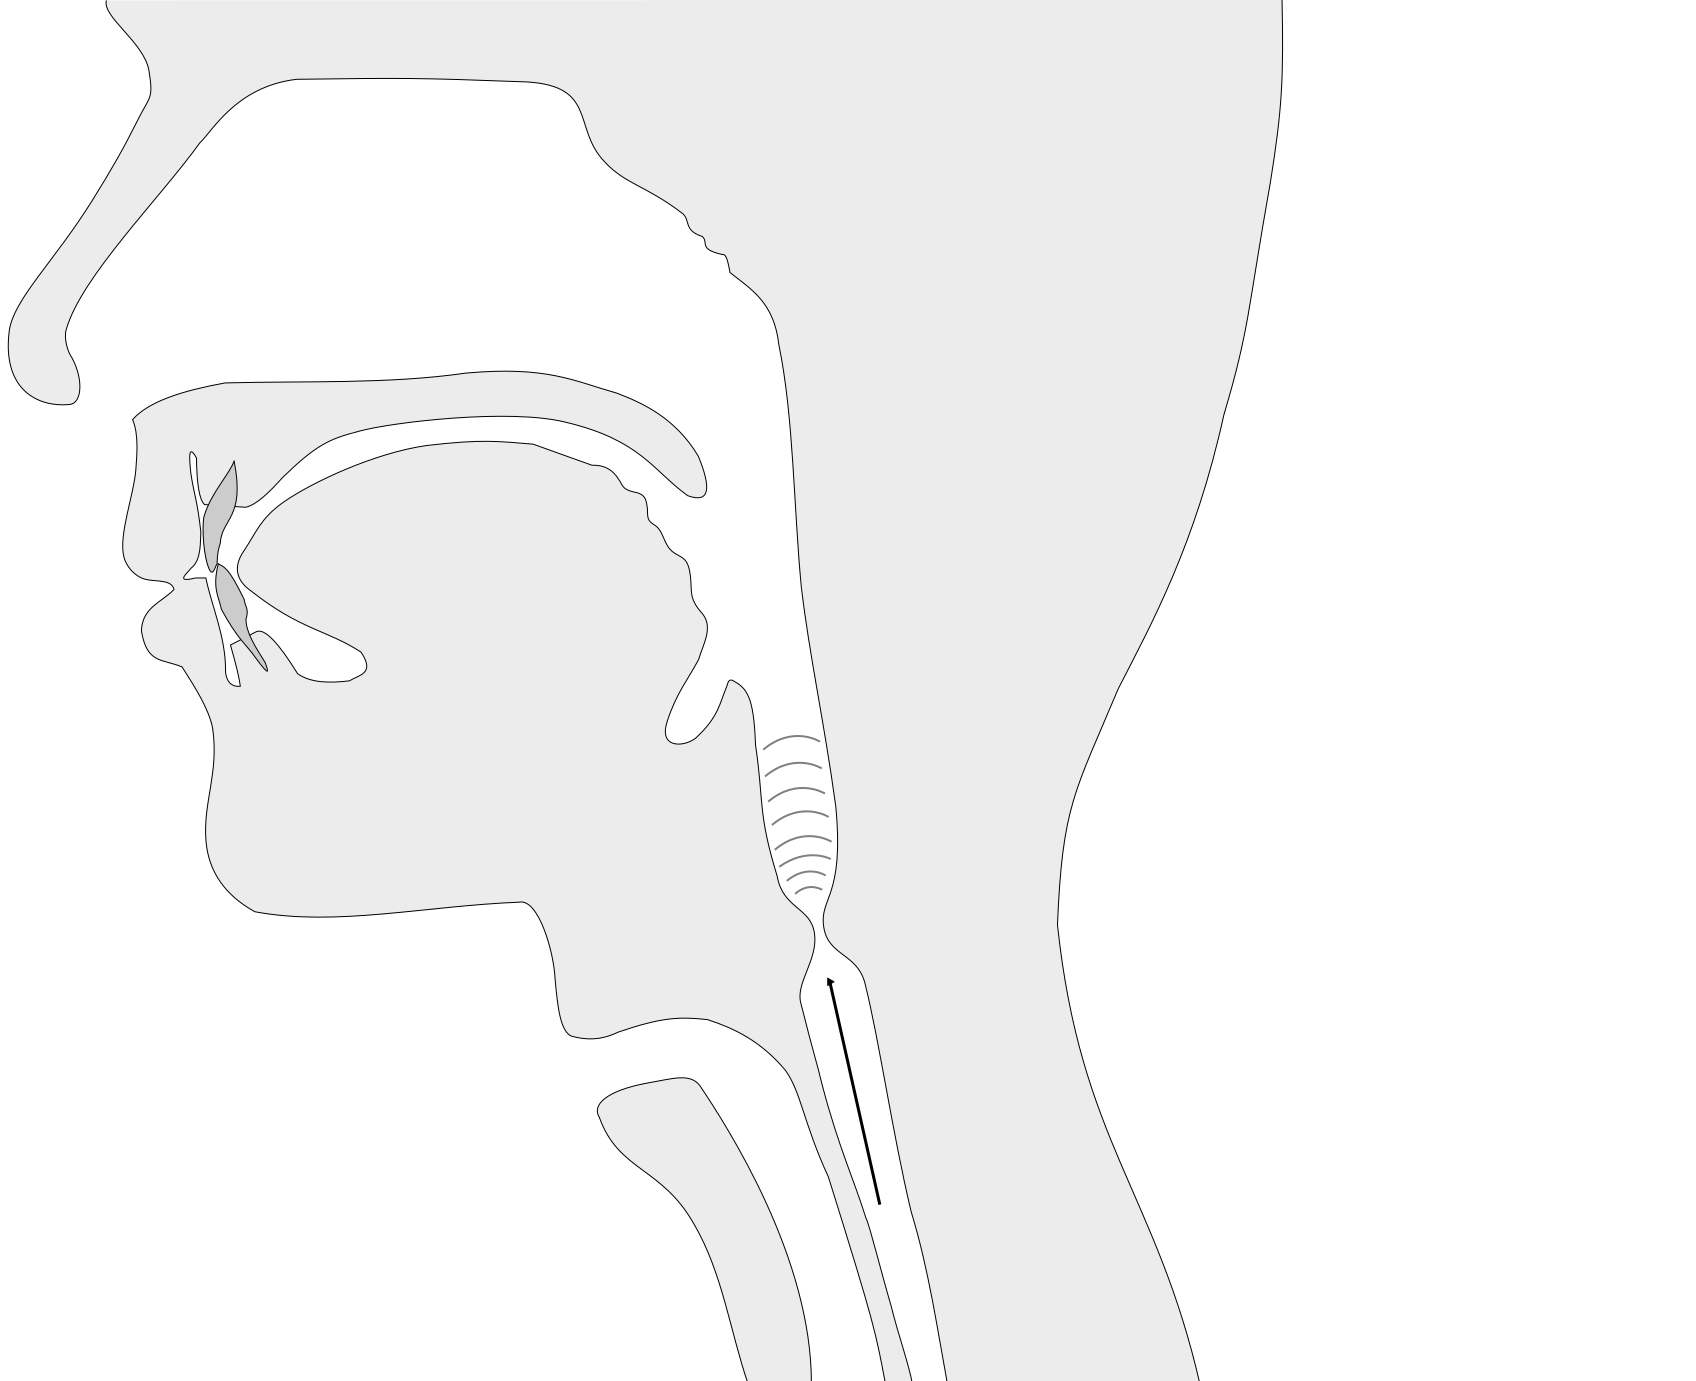
\includegraphics[width=0.6\linewidth]{ch3-cause/figures/esophageal}
%     \caption[Princip produkce jícnového hlasu.]{Princip produkce jícnového hlasu. Průchodem vzduchu přes zúžení vzniká základní tón jícnového hlasu.}
%     \label{fig:cause:treatment:esophageal}
%   \end{center}
% \end{figure}

% Na základě toho, jakým způsobem je jícen plněn vzduchem, rozlišujeme metodu \textbf{aspirační} a metodu \textbf{injekční}. Zatímco aspirační metoda spočívá v~plnění jícnu vzduchem pomocí polykání, u injekční metody je za tímto účelem využíván kořen jazyka, pomocí něhož je vzduch vtlačován do jícnu. Následný princip produkce hlasu je pro oba případy shodný. Injekční princip plnění jícnu vzduchem je využíván pacienty, kterým byla
% při laryngektomii odstraněna jazylka. V~těchto případech nelze jícen naplnit aspirační cestou.

% Proces učení jícnového hlasu by měl začít co možná nejdříve po operaci. Pokud
% je to možné, tak se s~výukou začíná ještě za pobytu pacienta na ORL klinice
% nebo krátce po propuštění. V~první fázi se pacient učí pouze slabiky
% sestávající z explosivy a souhlásky. Postupně se však přidávají slabičné
% shluky, které sice nedávají smysl, ale pomáhají v~osvojení potřebné techniky.
% V případě úspěšného zvládnutí se přistupuje  k~nácviku frází a souvislé řeči.
% Potřebnou dobu  k~nácviku jícnového hlasu nelze přesně určit, protože je
% závislá na mnoha faktorech. V~literatuře se uvádí, že pro úspěšné osvojení techniky jícnového hlasu je potřeba 30 až 50 hodin velmi intenzivního tréninku \cite{Brown2003}. Míra úspěšnosti nácviku srozumitelného hlasu se uvádí v~rozsahu 14\%-75\%. %Takto obrovský rozsah značí o mnoha faktorech, které mohou ovlivnit úspěšné osvojení jícnového hlasu.
% Mezi možné příčiny, které mohou významně ovlivnit zvládnutí techniky jícnového hlasu, patří
% fyziologické potíže, anatomické problémy, psychologické problémy, nebo jednoduše
% neadekvátní podpora při řečové terapii \cite{Brown2003}. Významnou roli také
% hraje snaha a odhodlání samotného pacienta.

% Nepopiratelnou výhodou využití metody jícnového hlasu je, že při rehabilitaci hlasu není pacient závislý na lékaři. Navíc po chirurgickém zásahu je zajištěno permanentní oddělení dýchacích a
% polykacích cest, je tedy eliminováno riziko vniknutí potravy do dýchacích cest.
% Další nespornou výhodou pro pacienty, kteří ovládají techniku jícnového hlasu, je bezesporu to, že mají při mluvení
% volné obě ruce. Za nevýhodu lze obecně považovat nižší srozumitelnost produkovaného hlasu.
% Ta je způsobena tzv. \uv{břišním} zabarvením, ke kterému zcela jistě při produkci řeči prostřednictvím metody jícnového hlasu  dochází, a dále nízkou intenzitou hlasu a krátkou výdrží mluvčího při tvorbě tónu. Za negativum se dá také považovat množství pacientem vynaloženého úsilí potřebného  k~osvojení
% techniky. Velmi často se také mluvčí ostýchají jícnový hlas používat, protože
% mají pocit, že je společensky nevhodné dorozumívat se formou blízkou říhání. Z
% tohoto důvodu se odhaduje, že v~běžném životě využívá jícnový hlas pouze 20\% -30\%
% pacientů, kteří se začali tuto techniku učit \cite{Hradecka2007}.

% subsubsection jícnový_hlas (end)

% \subsubsection{Využití elektrolarynxu} % (fold)
% \label{chap:cause:treatment:foniatric:elektrolarynx}

% Rehabilitace hlasu za pomoci přídavného zařízení, nazývaného elektrolarynx, se řadí mezi tzv. elektromechanické
% metody. Princip metody spočívá v~přikládání speciálního zařízení obsahujícího generátor zvuku do oblasti spodiny úst. Generátor zvuku, který je součástí elektrolarynxu, napomáhá přenosu zvuku a vibrací nejen do dutiny ústní, ale i do přilehlých artikulačních orgánů. Následně je pacient schopen běžným způsobem artikulovat, a tedy i hovořit. Princip vytváření hlasu pomocí elektrolarynxu je ukázán na obr. \ref{fig:cause:treatment:electrolarynx}.

% \begin{figure}[htb]
%   \begin{center}
%     
\includegraphics[width=0.6\linewidth]{ch3-cause/figures/electrolarynx}
%     \caption[Princip rehabilitace hlasu pomocí elektrolarynxu.]{Princip rehabilitace hlasu pomocí elektrolarynxu.}
%     \label{fig:cause:treatment:electrolarynx}
%   \end{center}
% \end{figure}

% Takto generovaná řeč se vyznačuje několika charakteristickými rysy. V~první
% řadě řeč budí velmi mechanický dojem. Důvodem je samozřejmě samotný
% elektrolarynx, který lze označit za elektromechanický generátor zvuku s
% konstantním buzením. Proto je také základní frekvence produkovaného hlasu víceméně konstantní a řečník tak má velmi omezené možnosti jak řeč emotivně zabarvovat. V~průběhu času se sice objevily snahy o ovlinění základní frekvence produkované řeči \cite{Kikuchi2004, Uemi1994, Goldstein2004}, kterou by bylo možné vyvolat prostřednictvím změny budící frekvence elektrolarynxu, ale ty ztroskotaly, jelikož jako velmi obtížné se jeví nalezení vhodného mechanismu, pomocí kterého by bylo docíleno optimální změny fundamentální frekvence mluvené řeči s~ohledem na to, co chce řečník říci. Dalším charakteristickým rysem hlasu produkovaného pomocí elektrolarynxu je jeho nižší srozumitelnost. K tomuto jevu dochází v~důsledku přítomnosti zvukového podkresu generovaného přístrojem. Srozumitelnost se navíc snižuje s~rostoucím okolním hlukem, proto se velmi často stává, že posluchač, který se s~takto produkovanou řečí setkává poprvé, není schopen promluvám plně porozumět.

% Naproti tomu, za výhody, kterými tato metoda rehabilitace hlasu disponuje, lze označit možnost rychlého
% osvojení schopnosti opětovně produkovat řeč. Navíc je vhodná pro téměř všechny pacienty
% postižené ztrátou hlasu v~důsledku odstranění hrtanu popř. jeho poškození.
% Za nevýhodu lze obecně pokládat kvalitu produkované řeči, tedy monotonní a
% mechanicky znějící hlas. Za jistý způsob omezení lze považovat nutnost držení elektrolarynxu, jakožto přídavného zařízení, při mluvení.

% \subsection{Chirurgicko-protetická metoda} % (fold)
% \label{chap:cause:treatment:tracheo}

% Další možností, kterou lze využít pro rehabilitaci hlasu, je po odstranění hrtanu chirurgicky vytvořit průchod
% mezi průdušnicí a jícnem tak, aby u tracheostomovaného člověka mohl opětovně proudit vzduch z plic do úst.
% Princip metody spočívá v~tom, že pacient při výdechu zneprůchodní operativně vytvořený otvor (stoma) v~oblasti krku. Vzduch tak projde skrz fistuli do oblasti jícnu, naráží do jeho stěn a dochází  k~jeho rozvibrování. Následně jsou tyto vibrace modulovány pomocí artikulačních orgánů a vzniká řeč.

% Historicky první zmínka o vytvoření fistule\footnote{fistule (česky píštěl) je abnormální
% otvor mezi dvěma dutými orgány, nebo mezi dutým orgánem a kůží.} mezi
% průdušnicí a jícnem pochází z~roku 1932. V~tomto roce doktor Guttman poprvé
% vytvořil tracheoezofageání shunt\footnote{shunt - kanál, kterým je tekutina
% odkloněna z přirozené dráhy. Tento kanál může být vytvořen chirurgicky nebo pomocí syntetické trubice. }.
% Hlavní snahou chirurgů bylo vytvoření bezpečné, správně nasměrované píštěle
% umožňující tvorbu hlasu. Bohužel v~mnoha případech byly zákroky doprovázené
% vážnými komplikacemi (infekcemi, zápaly či těžkým krvácením).
% Mimo to se museli operatéři vypořádat se zajištěním stálosti
% vytvořeného otvoru tak, aby jím neprotékaly tekutiny špatným směrem a
% nedocházelo  k~jejich zatékání do dýchacích cest. Jelikož se jednalo o velmi
% náročné operační postupy a bylo s~nimi spojeno velké množství rizik, došlo v
% 80.~letech 20.~století  k~jejich ústupu. Svou renesanci zažily s~návrhem první protézy v~podobě jednocestného ventilu, který zajišťoval pouze jednosměrný
% průchod tekutin skrze píštěl, jak je ilustrováno na obr.
% \ref{fig:cause:treatment:shunt}. První komerčně dostupná protéza se objevila
% v~80.~letech 20.~století v~USA.

% \begin{figure}[htb]
%   \begin{center}
%     
\includegraphics[width=0.6\linewidth]{ch3-cause/figures/te-shunt}
%     \caption[Průchod vzduchu tracheoezofageální protézou.]{Průchod vzduchu tracheoezofageální protézou.}
%     \label{fig:cause:treatment:shunt}
%   \end{center}
% \end{figure}

% Na používané protézy jsou kladené
% přísné nároky a musí vyhovovat určitým požadavkům. Musí být vyrobeny
% z~biokompatibilního materiálu, který odolává biodegradaci. Tím je zaručena jejich
% dlouhodobá trvanlivost a správná funkce. V~neposlední řadě by měla být protéza
% samofixační a snadno vyměnitelná.
%  K zajistění jejich správné funkce je zapotřebí navrhnout je tak, aby
% tlak potřebný  k~otevření faryngoezofageálního segmentu byl co nejnižší. To by mělo zajišťovat pacientovi vytvářet
% plynulou řeč. První vyráběné protézy se ale vyznačovaly tím, že tlak potřebný pro jejich otevření byl příliš vysoký a omezovaly tak množinu potencionálních pacientů. Nejmodernější protézy se již vyznačují
% velmi nízkým otevíracím fonačním tlakem.

% V praxi se používá několik druhů protéz. Hlavním rozdílem mezi nimi však je,
% zda se pacient přímo účastní výměny ventilu, jehož fundamentální funkcí je
% vytvoření průchodu pro vzduch proudící z průdušnice do jícnu. U protéz, které
% jsou vyměňovány operačně, se doba používání pohybuje od 3 do 6 měsíců. Tento
% interval velmi významně ovlivňuje tvorba biofilmu na povrchu náhrady. K tvorbě
% dochází následkem přímého kontaktu protézy s~tělními tekutinami a potravou.
% Rychlost tvorby biofilmu ovlivňuje tvar a materiál, ze kterého je náhrada
% vytvořena \cite{Leunisse2001}. U typů, které si nositel může měnit sám, se
% předpokládá, že budou čištěny nebo měněny přibližně jednou za dva týdny. Na obr. \ref{fig:cause:treatment:prosthesis} jsou
% ukázány některé typy užívaných protéz.

% \begin{figure}[htb]
%   \begin{center}
%     \includegraphics[width=0.9\linewidth]{ch3-cause/figures/te-protezy}
%     \caption[Ilustrace používaných TE protéz.]{Ilustrace používaných TE protéz (a) Gronigenova nízkotlaká protéza, (b) Provox2 a (c) Blom-Singer protéza.}
%     \label{fig:cause:treatment:prosthesis}
%   \end{center}
% \end{figure}

% Samotný zákrok zavedení protézy je možné provést současně s~výkonem totální
% laryngektomie (tzv. primární zavedení hlasové protézy) nebo až po zotavení
% pacienta z~náročné léčby nádorového onemocnění (tzv. sekundární zavedení).
% Primární zavedení umožňuje začít s~hlasovou rehabilitací krátce po odstranění
% hrtanu. Zároveň pacient nemusí v~krátké době podstupovat druhou operaci, při
% které by se vkládal jednocestný ventil do vytvořené fistule.

% V praxi se ukázalo, že úspěšnost rehabilitace pomocí této metody je více než 80~\%
% \cite{Slavicek2002}. Důležitým faktorem, stejně jako u metody jícnového hlasu, je
% funkčnost faryngoezofageálního segmentu. Významnou roli hraje také otvírací tlak horního
% jícnového svěrače. Hlas tvořený protézou se vyznačuje vysokou kvalitou, dobrou
% srozumitelností, individuálním zabarvením a relativně dlouhou fonační dobou
% dosahující průměrně 20 sekund \cite{Saito2003}. Oproti jícnovému hlasu není potřeba
% tak intenzivní edukace pacienta k~plnému osvojení hlasu. V~současnosti se
% jedná o nejpoužívanější metodu rehabilitace hlasu.

% \subsection{Hrtanu podobné struktury} % (fold)
% \label{chap:cause:tratment:structure}

% S rozvojem mikrovaskulárních\footnote{mikrovaskulární - část oběhového systému
% složeného z nejmenších cév, jako jsou kapiláry, žilky aj.} transplantátů se
% začaly objevovat postupy, které umožňovaly rehabilitovat hlas pouze pomocí
% chirurgického zákroku. Tyto techniky jsou založeny na myšlence permanentního spojení hypofaryngu
% s tracheou pomocí vlastní tkáně pacienta.

% První metodu tohoto druhu představil v~roce 1984 doktor Ehrenberger
% \cite{Kramp2009}, který popsal tzv. \uv{\textbf{řečový sifón}}
% (angl. \textbf{speech siphon}). Jedná se o dvakrát esovitě zahnuté spojení mezi hrtanem a hltanem
% vytvořené z části tenkého střeva zvané lačník (jejunum). Dvojesovité zahnutí je provedeno tak, aby
% bylo minimalizováno riziko sekundární aspirace. Schéma \uv{řečového sifónu}
% podle Ehrenberga je znázorněno na obr. \ref{fig:cause:treatment:microvascular}
% A. Již na první pohled je zřejmé, že se jedná o velmi náročný chirurgický
% zákrok. První články publikované autorským kolektivem prezentovaly velmi dobré
% funkční výsledky metody. Podle \cite {Sebova-Sedenkova2006} bylo touto metodou doposud
% operováno přibližně 60 pacientů.

% V roce 1990 byla popsána laryngoplastika podle Hagena. V~tomto případě je za účelem vytvoření ústrojí zvaného \textbf{neolarynx} používán štěp z předloktí. Neoglottis je vyztužen chrupavkou
% a překrývá vchod do neolaryngu tak, aby nedocházelo  k~sekundární aspiraci. Vnitřek neolaryngu je kryt kůží.
% Laryngoplastika podle Hagena je znázorněna na obr.
% \ref{fig:cause:treatment:microvascular} B. Doposud bylo touto metodou operováno přibližně 300
% pacientů \cite{Sebova-Sedenkova2006}.

% \begin{figure}[htb]
%   \begin{center}
%     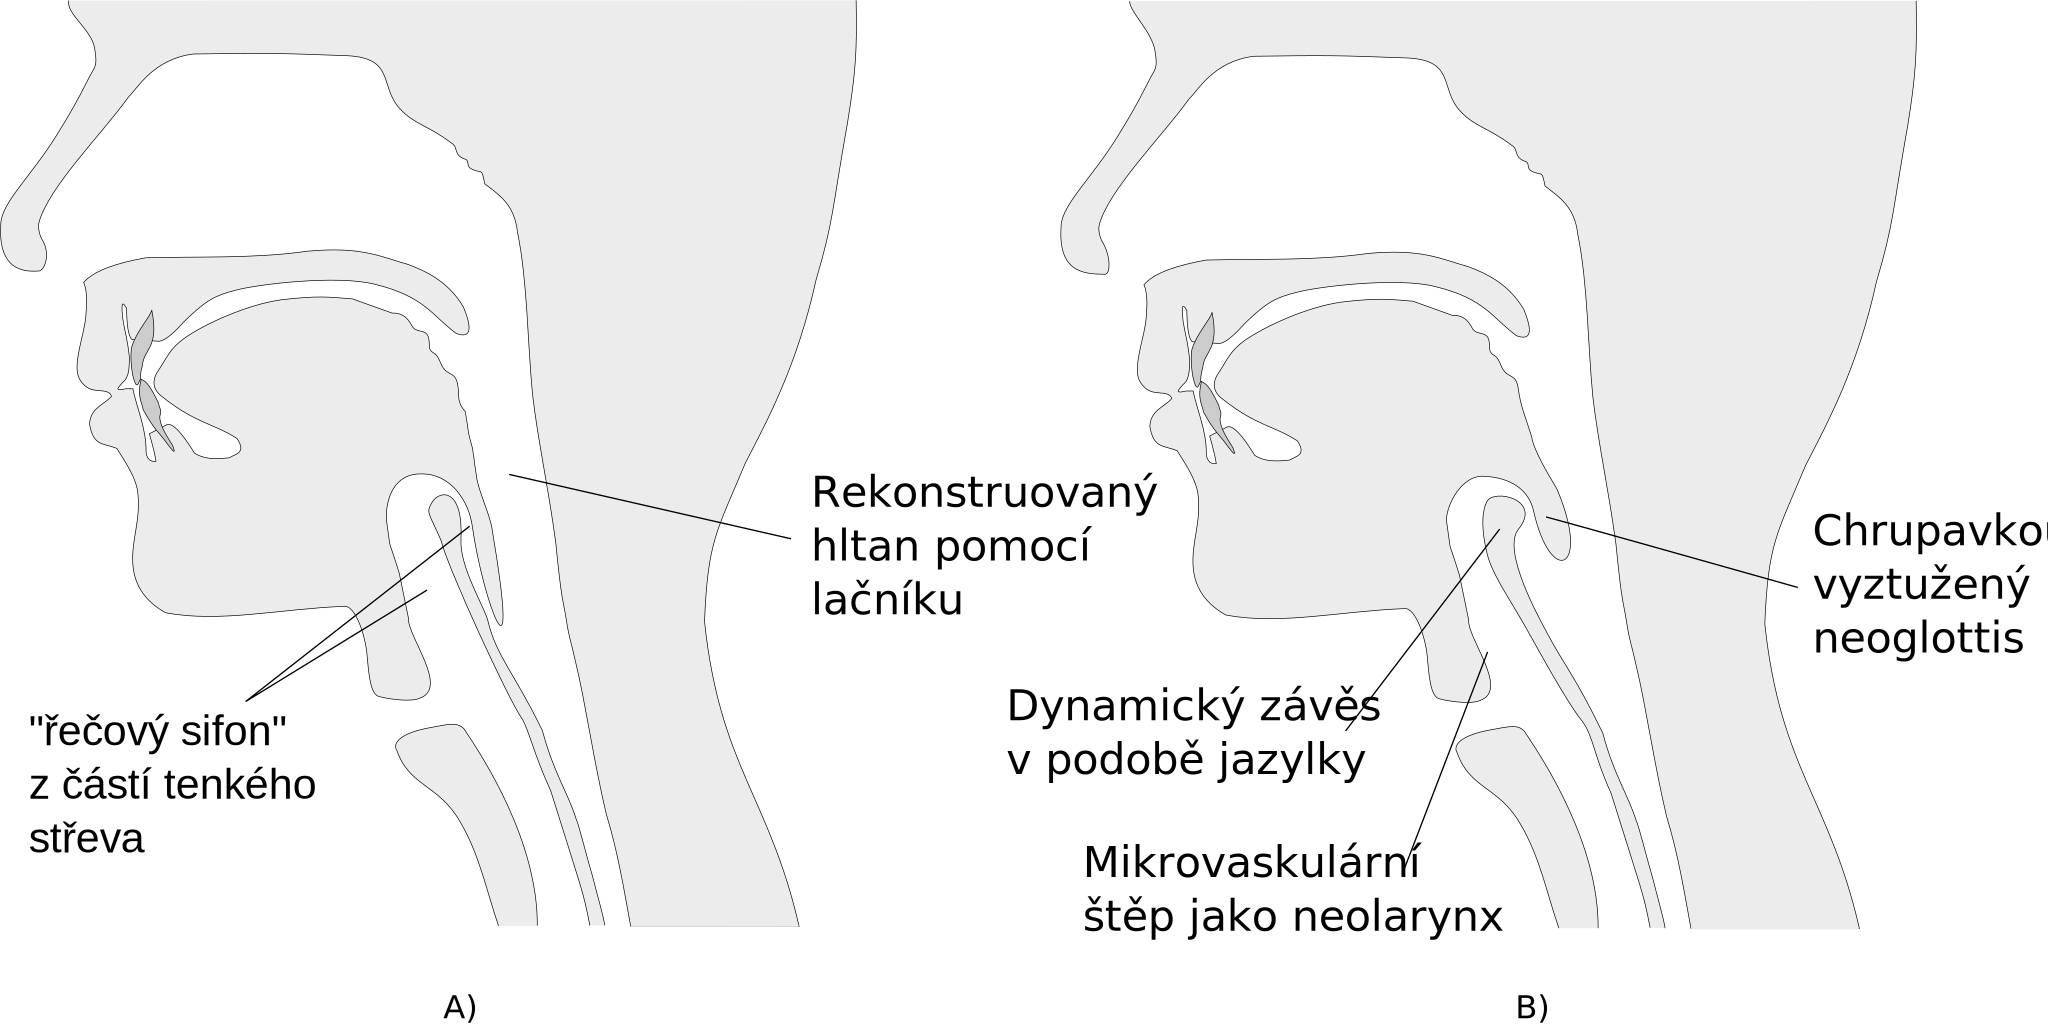
\includegraphics[width=0.9\linewidth]{ch3-cause/figures/microvascular}
%     \caption[Schéma \uv{řečového sifónu} a laryngoplastiky.]{A) Schéma \uv{řečového sifónu} tak jak jej představil Ehrenberg. B) Laryngoplastika podle Hagena.}
%     \label{fig:cause:treatment:microvascular}
%   \end{center}
% \end{figure}

% Bohužel v~současné době tyto metody nenacházejí širší uplatnění. Hlavním důvodem je
% náročnost realizace operačních postupů, kvůli které se velmi
% těžko prosazují na dalších pracovištích. Dalším aspektem, který limituje tyto
% metody, je vliv na samotného pacienta. Metody předpokládají provedení dalšího chirurgického
% zákroku, který představuje pro pacienta další zátěž a mohou ho provázet nemalé komplikace.
% I přes nedostatky těchto metod je
% pochopitelná snaha lékařů o intenzivní výzkum v~této oblasti. Při úspěšné
% léčbě je pacient schopen produkovat hlas velmi dobré kvality a ve většině
% případů nepotřebuje žádnou péči ze strany lékařů.

% \subsection{Transplantace hrtanu}
% \label{chap:cause:treatment:transplantation}

% Nejkomplexnější možnost rehabilitace hlasu představuje transplantace hrtanu.
% Pokud je úspěšná, přebírá transplantovaný orgán plně funkci původního
% orgánu a velmi významně zvyšuje šance pacienta na plné zotavení bez trvalých
% následků. Jedná se ale o velmi náročný chirurgický zákrok, protože je potřeba provést reinervaci a obnovení cévního zásobení implantátu.

% Přestože první zmínky o možnosti provedení transplantace hrtanu se objevují již v~60.~letech 20.~století\footnote{Vůbec první úspěšná transplantace
% orgánu (ledvin) se uskutečnila v~roce 1954.}, byla první transplantace tohoto druhu provedená
% až profesorem Marshallem Stromem v~roce 1998 \cite{Narula2011},
% Prvním pacientem, který podstoupil zmiňovaný chirurgický zákrok, byl čtyřicetiletý muž z USA.
% K~laryngektomii v~jeho případě vedla motocyklová nehoda, při které došlo  k~rozdrcení hrtanu. Před transplantací pacient využíval 20 let  k~produkci řeči elektrolarynx. Dárcem orgánu byl taktéž čtyřicetiletý muž, který zemřel na následky prasknutí mozkového aneurysmatu. Příjemce transplantátu již třetí den po operaci promluvil (vyslovil
% anglické slovo \uv{hello}). Přibližně po 36 měsících od transplantace byl
% produkovaný hlas kvalitativně srovnatelný s~hlasem zdravého člověka. U této transplantace se však nepodařilo dosáhnout kompletní reinervace, proto nebylo možné zajistit bezproblémové dýchání a bylo proto nutné
% ponechat tracheostomii. I přes tuto skutečnost měl zákrok významný podíl na zvýšení kvality jeho života
% \cite{Strome2001}. Doposud poslední úspěšně vykonaná transplantace hrtanu byla
% dle dostupných zdrojů provedena v~říjnu 2010.

% Jedním z hlavních důvodů tak nízkého počtu úspěšně provedených zákroků je, že se jedná o transplantaci dárcovského orgánu. Pacientům jsou podávány medikamenty zabraňující odmítnutí dárcovského orgánu (imunosupresiva), která ale v~současné době nelze podávat pacientům trpícím rakovinným onemocněním, protože významně zvyšují riziko opětovného rozšíření rakoviny \cite{Narula2011}. Ve výjimečných případech lze tuto metodu zvažovat u pacientů, kteří trpěli benigními nádory a minimálně 5~let u nich nedošlo  k~recidivě.
% Poslední výzkumy však naznačují, že by v~dohledné době v~této oblasti mohlo dojít  k~pokroku, v~důsledku kterého by bylo možno provést transplantaci hrtanu i u lidí, kteří trpěli rakovinným onemocněním.

% \subsection{Shrnutí} % (fold) \label{sub:treatment:summary}

% Rehabilitaci hlasu u pacientů, kteří prodělali chirurgické odstranění hrtanu, je ve
% vyspělých zemích věnována značná pozornost, jelikož následky této operace velmi významně ovlivňují kvalitu jejich života. Léčení jedinci se musí vyrovnat primárně se ztrátou hlasu. V~některých případech dochází po operaci i ke ztrátě čichu a pacienti jsou náchylnější ke vzniku respiračních onemocnění.
% Tato situace je již sama o sobě velmi náročnou psychickou zkouškou. Neméně významnou
% roli sehrává i fyzická odlišnost a z~toho pramenící psychická zátěž, které je pacient vystaven
% po absolvované léčbě.

% V~současnosti je za účelem rehabilitace hlasu využíváno několik metod, jejichž
% Souhrnný přehled spolu s~hlavními výhodami a nevýhodami jednotlivých rehabilitačních přístupů je uveden v~tab. \ref{tab:treatment:summary}.
% U většiny pacientů je hlas rehabilitován pomocí metody tracheoezofageálního píštěle,
% která je principiálně založena na metodě jícnového hlasu. O úspěchu rehabilitace, stejně jako u jícnového hlasu, tak
% především rozhodují vlastnosti faryngoezofageálního segmentu. Pokud si pacient
% není schopen osvojit techniku jícnového hlasu, případně nemá voperován píštěl, je
% pro rehabilitaci hlasu použit elektrolarynx. Za nejkomplexnější ze zmíněných postupů se dá považovat úplná transplantace hrtanu, která
% řeší víceméně všechny problémy spojené s~odstraněním hrtanu. Bohužel tento
% zákrok je velmi náročný a vhodný pouze pro omezený okruh pacientů.

\newcolumntype{b}{X}
\newcolumntype{s}{>{\hsize=.5\hsize}X}

\begin{table}[ht]
  \centering
  \begin{tabularx}{1.0\textwidth}{L{1.2} L{0.6} L{1.1} L{1.1}}
    & \textbf{Kvalita} & \textbf{Výhody} & \textbf{Nevýhody} \\
    \toprule \\ [-1.75ex]

    \textbf{Tracheoezofageální píštěl} & Vysoká & Vysoká míra osvojení, dlouhá fonační doba & Zanášení píštěle a s~ním spojené čištění, případně dodatečná lékařská péče \\
    \midrule \\ [-1.75ex]

    \textbf{Jícnový hlas} & Dobrá & Volné ruce při mluvení, není potřeba dodatečné lékařské péče & Velmi náročná metoda  k~naučení, nepřirozený hlas \\
    \midrule \\ [-1.75ex]

    \textbf{Elektrolarynx} & Nízká & Snadné  k~naučení & Monotonní až robotický hlas, nutné nosit externí elektrické zařízení \\
    \midrule \\ [-1.75ex]

    \textbf{Hrtanu podobné struktury} & Vysoká & Nezávislost pacienta na pravidelné lékařské péči & Velmi náročná chirurgická procedura, která pacienta vystavuje dalším možným rizikům  \\
    \midrule \\ [-1.75ex]

    \textbf{Transplantace hrtanu} & Velmi vysoká & Transplantovaný hrtan přejímá funkci odstraněného orgánu & Velmi náročná chirurgická procedura, která je vhodná jen pro malé procento pacientů \\
  \end{tabularx}

  \caption{Přehled dostupných metod rehabilitace hlasu. \label{tab:treatment:summary}}
\end{table}

% Přestože lékařská věda v~současnosti disponuje možnostmi jak rehabilitovat hlas a lékaři se snaží využívané postupy neustále zdokonalovat, zůstává zde otevřený prostor pro inovace, a tím zlepšení kvality života lidí postižených ztrátou hrtanu.

